%%%%%%%%%%%%%%%%%%%%%%%%%%%%%%%%%%%%%%%%%
% Beamer Presentation
% LaTeX Template
% Version 1.0 (10/11/12)
%
% This template has been downloaded from:
% http://www.LaTeXTemplates.com
%
% License:
% CC BY-NC-SA 3.0 (http://creativecommons.org/licenses/by-nc-sa/3.0/)
%
%%%%%%%%%%%%%%%%%%%%%%%%%%%%%%%%%%%%%%%%%

%----------------------------------------------------------------------------------------
%	PACKAGES AND THEMES
%----------------------------------------------------------------------------------------

\documentclass{beamer}

\mode<presentation> {

% The Beamer class comes with a number of default slide themes
% which change the colors and layouts of slides. Below this is a list
% of all the themes, uncomment each in turn to see what they look like.

%\usetheme{default}
%\usetheme{AnnArbor}
%\usetheme{Antibes}
%\usetheme{Bergen}
%\usetheme{Berkeley}
%\usetheme{Berlin}
%\usetheme{Boadilla} %like
%\usetheme{CambridgeUS}
%\usetheme{Copenhagen}
%\usetheme{Darmstadt}
%\usetheme{Dresden}
%\usetheme{Frankfurt}
%\usetheme{Goettingen} %like
\usetheme{Hannover} %like
%\usetheme{Ilmenau}
%\usetheme{JuanLesPins}
%\usetheme{Luebeck}
%\usetheme{Madrid}
%\usetheme{Malmoe}
%\usetheme{Marburg}
%\usetheme{Montpellier}
%\usetheme{PaloAlto}
%\usetheme{Pittsburgh}
%\usetheme{Rochester}
%\usetheme{Singapore}
%\usetheme{Szeged}
%\usetheme{Warsaw}

% As well as themes, the Beamer class has a number of color themes
% for any slide theme. Uncomment each of these in turn to see how it
% changes the colors of your current slide theme.

%\usecolortheme{albatross}
%\usecolortheme{beaver}
%\usecolortheme{beetle}
%\usecolortheme{crane}
%\usecolortheme{dolphin}
%\usecolortheme{dove}
%\usecolortheme{fly}
%\usecolortheme{lily}
%\usecolortheme{orchid}
%\usecolortheme{rose}
%\usecolortheme{seagull}
%\usecolortheme{seahorse}
%\usecolortheme{whale}
%\usecolortheme{wolverine}

%\setbeamertemplate{footline} % To remove the footer line in all slides uncomment this line
%\setbeamertemplate{footline}[page number] % To replace the footer line in all slides with a simple slide count uncomment this line

%\setbeamertemplate{navigation symbols}{} % To remove the navigation symbols from the bottom of all slides uncomment this line
}

\usepackage{graphicx} % Allows including images
\usepackage{booktabs} % Allows the use of \toprule, \midrule and \bottomrule in tables
\usepackage{pgfpages}
\usepackage{amsmath}
\usepackage{pgfplots}
\usepackage{tikz}
\usepackage{xcolor}

%----------------------------------------------------------------------------------------
%	TITLE PAGE
%----------------------------------------------------------------------------------------

\title[Computation \& optimization]{Computation \& optimization for Lasso - part 2} % The short title appears at the bottom of every slide, the full title is only on the title page

\author{Luyang Han \& Janosch Ott} % Your name
\institute[] % Your institution as it will appear on the bottom of every slide, may be shorthand to save space
{
ETH Zürich \\ % Your institution for the title page
%\medskip
%\textit{john@smith.com} % Your email address
}
\date{22 October 2018} % Date, can be changed to a custom date

\setbeamercovered{transparent} % else hidden elements are gray, this way they are invisible
\setbeamertemplate{navigation symbols}{} %comment to have a lot of navigating symbols
\setbeamertemplate{section in toc}[sections numbered] % removes the ugly balls
%\setbeameroption{show notes}
%\setbeameroption{show notes on second screen=right}
%\setbeameroption{show only notes}

\setbeamertemplate{enumerate items}[default] % to get rid of some more ugly balls


%%%%%%%% ------------%%%%%%%%%%-----------%%%%%%%%%%%------------%%%%%%%%%%-----------
\newcommand{\R}{\mathbb{R}}
\newcommand{\Norm}[1]{\left\lVert#1\right\rVert}
\newcommand{\norm}[1]{\left\lvert#1\right\rvert}
\DeclareMathOperator*{\argmin}{arg\,min}
\DeclareMathOperator*{\argmax}{arg\,max}



%%%%%%%%%%% ----------%%%%%%%%%%-----------%%%%%%%%%%------------%%%%%%%%%--------------


\usepackage{hyperref}



\begin{document}

\begin{frame}
\titlepage % Print the title page as the first slide
\end{frame}

\begin{frame}
\frametitle{Overview} % Table of contents slide, comment this block out to remove it
\tableofcontents % Throughout your presentation, if you choose to use \section{} and \subsection{} commands, these will automatically be printed on this slide as an overview of your presentation
\end{frame}

%----------------------------------------------------------------------------------------
%	PRESENTATION SLIDES
%----------------------------------------------------------------------------------------


%------------------------------------------------
\section{Coordinate Descent}
%------------------------------------------------
\begin{frame}
\frametitle{Coordinate Descent Algorithm}
\begin{block}{What is Coordinate Descent (CD) Algorithm?}
\begin{equation}    % <--- deleted empty lines
            \beta^{t+1}_{k} = \underset{\beta_k}{\mathrm{argmin}}\ f(\beta^{t}_{1}\ ,\beta^{t}_{2}\ ,...\beta_{k}\ ,\beta^{t}_{k+1}\ , ...\beta^{t}_{p})
    \end{equation}
    \; and $\beta^{t+1}_j =\ \beta^{t}_j$ for $j \neq k$
    \vspace*{6mm}
\begin{itemize}
\item  An iterative algorithm that updates from $\beta^t$ \ to \   $\beta^{t+1}$ \  by choosing a single coordinate, and minimizing over this coordinate.
\end{itemize}
\end{block}
\end{frame}

\begin{frame}
\frametitle{Separability Condition}
\textbf{Motivation} 
\vspace*{6mm}
\begin{block}{Does CD procedure converge to the global minimum of a convex function? }
\vspace*{3mm}
\only<2> {
\begin{itemize}
    \item \textbf{Sufficient Condition:}\  the function is continuously differentiable and strictly convex in each coordinate. 
\end{itemize}
$\Rightarrow$  restrictive 

}

\end{block}
\note{restrictive regarding its application to Lasso, regularizers leads to optimization problems that need not be differentiable.}
    
\end{frame}

\begin{frame}{Separability Condition}
Suppose the cost function \(f\) has the additive decomposition:
\begin{equation}
    f(\beta_1,...,\beta_p)=g(\beta_1,...,\beta_p)+\displaystyle\sum_{j=1}^{p} h_j(\beta_j)
\end{equation}
where \(g:\mathbb{R}^p \rightarrow \mathbb{R}\) is differentiable and convex, and the univariate functions  \(h_j:\mathbb{R} \rightarrow \mathbb{R}\) is convex. 
\vspace*{6mm}
\begin{itemize}
    \item \underline{Lasso}: \(g(\beta)=\frac{1}{2N}{\lVert\textbf{y}-\textbf{X}\beta\rVert}^2_2 \) and \(h_j(\beta_j)=\lambda\lvert\beta_j\lvert\) satisfies the condition
\end{itemize}
    
\end{frame}


\begin{frame}{Separability Condition: Example}
An Example of failure of Coordinate Descent 


\vspace*{6mm}
\(\underset{\beta\in\mathbb{R}^p}{\mathrm{argmin}}\ \frac{1}{2N}{\lVert\textbf{y}-\textbf{X}\beta\rVert}^2_2 + \ \lambda_{1}\sum_{j=1}^{p}\lvert\beta_j\lvert+\ \lambda_{2}\sum_{j=2}^{p}\lvert\beta_j-\beta_{j-1}\lvert\)

\vspace*{6mm}
\begin{itemize}
    \item \(h(\beta)\) is not separable
\end{itemize}
\begin{itemize}
    \item Fused Lasso: coordinate descent procedure is not guaranteed to find the global minimum
\end{itemize}


    
\end{frame}


\begin{frame}{Separability Condition: Example}
\begin{figure}[h]
\centering
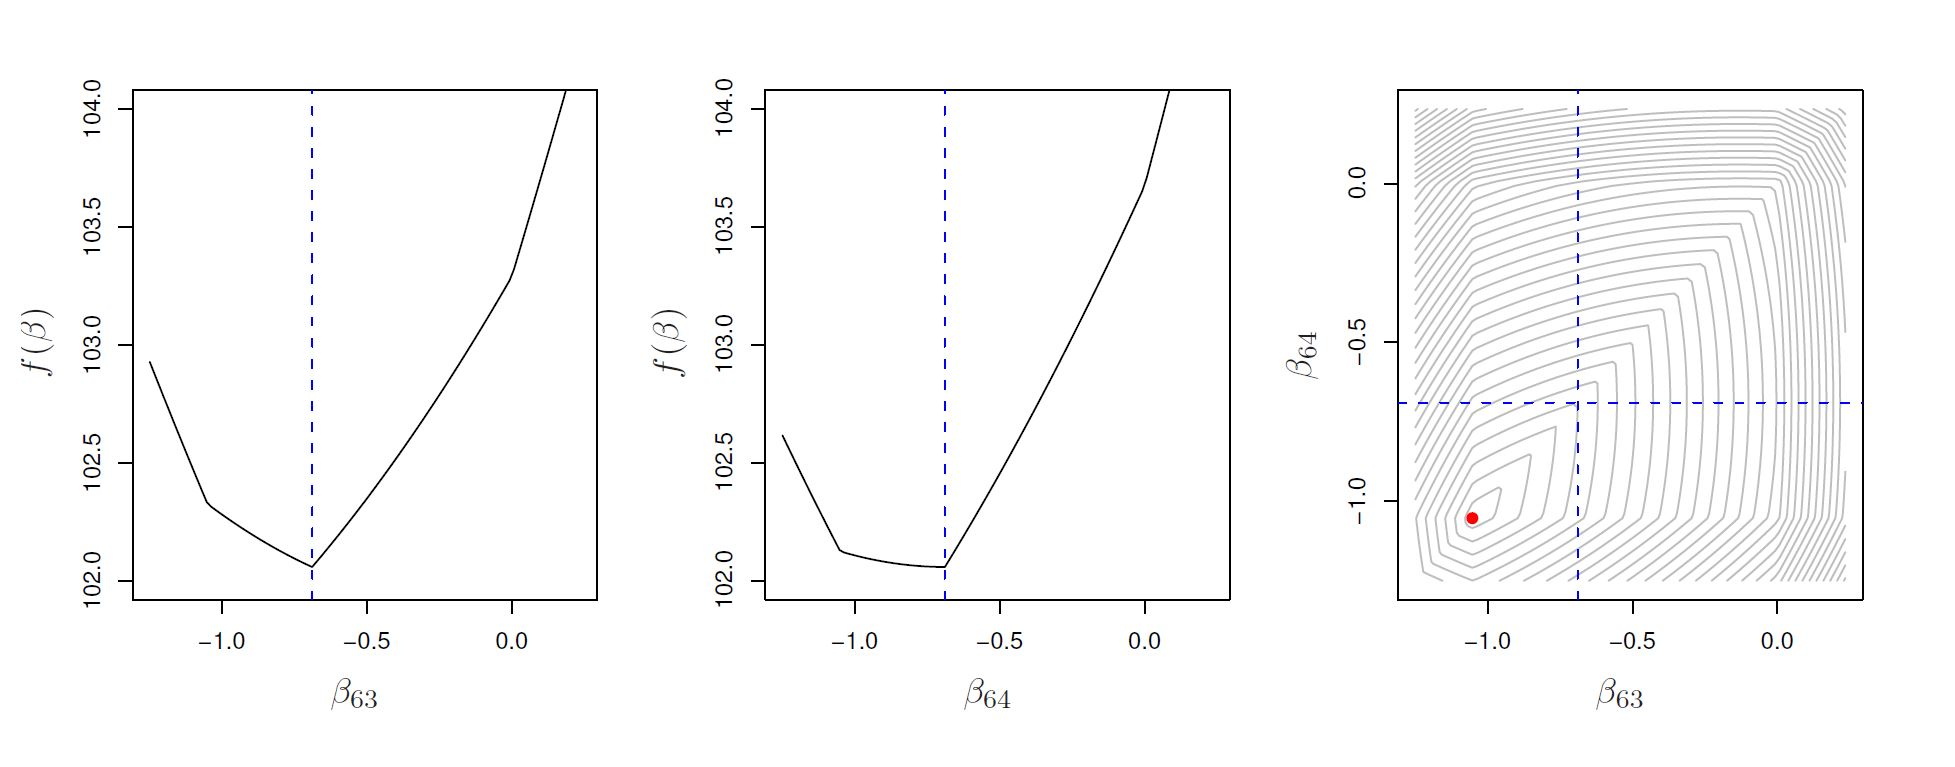
\includegraphics[width=10cm]{img/Fused}
\caption{ Fused Lasso: CD fail to reach the global minimum}
\end{figure}
 \footnote{Picture taken from \textit{Statistical Learning with Sparsity}  page 111 }
\end{frame}

\begin{frame}{Lasso \& Coordinate Descent}

\textbf{Optimality Condition:}
\vspace*{4mm}

\(-\frac{1}{2N}\sum_{i=1}^{N}(y_{i}-\beta_0-\sum_{k=1}^{p}x_{ik}\beta_k)x_{ij}+ \lambda s_j=0\)
\vspace*{4mm}
 \\where \(s_j \in sign(\beta_j)\) for \(j=1,2,...p\)
 \vspace*{6mm}
 \begin{itemize}
     \item Define the \textbf{partial residual}: \(r_{i}^{(j)}=y_i-\sum_{k\neq j}x_{ik}\hat{\beta}_k\)
    \item Then the solution for \(\hat{\beta_j}\) satisfies:\\
\vspace*{4mm}
    \(\hat{\beta_j}=\frac{S_{\lambda}(\frac{1}{N}\sum_{i=1}^{N}r_i^{(j)}       x_{ij} )}{\frac{1}{N}\sum_{i=1}^{N}x_{ij}^2}\)\\
\vspace*{4mm}
    where \(S_{\lambda}(\theta) =sign(\theta)(\lvert\theta\lvert-\lambda)_{+}\)
\end{itemize}
    
\end{frame}




\begin{frame}{Lasso \& Coordinate Descent}
\begin{itemize}
    \item Illustration of Coordinate Descent in R
\end{itemize}
\begin{block}{Strategies to make the operation efficient: }
\vspace*{3mm}  
\textbf{Naive Updating} \\
\vspace*{1.5mm}
\(r_i^{(j)}=y_i-\sum_{k\neq j}x_{ik} \hat{\beta}_k = r_i + x_{ij}\hat{\beta }_j\) \\
\vspace*{1.5mm}
\(\frac{1}{N} \sum_{i=1}^{N}x_{ij}r_i^{(j)} = \frac{1}{N} \sum_{i=1}^{N} x_{ij}r_i + \hat{\beta}_j\) \\
\vspace*{3mm}  
\textbf{Covariance Updating} \\
\vspace*{1.5mm}

        \(\sum_{i=1}^{N}x_{ij}r_{i}= \big \langle x_j,y\big\rangle -  \sum_{k\lvert \lvert \beta_{\hat{k}}\rvert >0}\big \langle x_j,x_k\big\rangle \beta_{\hat{k}}\) \\
\vspace*{3mm}      
\textbf{Warm Starts}:  For a decreasing sequence of values $\{\lambda_{0}^{L}\}$, \(\hat{ \beta}(\lambda_l)\) is typically a
very good warm start for the solution $\hat{ \beta}(\lambda_{l+1})$. \\
We set $\lambda_0 = \frac{1}{N} max|\langle x_j, y \rangle|$ and $\lambda_L \approx 0 $
\end{block}
    
\note{\textbf{Covariance updating}: In this approach, we compute inner products of each feature with y initially,and then each time a new feature xk enters the model for the first time, wecompute and store its inner product with all the rest of the features, requiringO(Np) operations. We also store the p gradient components. If one of the coefficients currently in the model changes, we can update each gradient in O(p) operations. Hence with k nonzero terms in the model, a complete cycle costs O(pk) operations if no new variables become nonzero, and costs O(Np) for each new variable entered. Importantly, each step does not require making.
O(N) calculations; \textbf{Warm Starts}: sequence of lambda values; double number of L, would not double the computational time; fewer iteration for each lambda. }
\end{frame}

\begin{frame}{Lasso \& Coordinate Descent }

\textbf{Active-set Convergence:} Define the
active set $A$ and iterate the algorithm using only  variables in $A$.\\
\vspace*{3mm}
\textbf{Strong-set Convergence:}  Define the strong set $S$ and iterate the algorithm using only variables in $S$.\\
\vspace*{3mm}
\textbf{Sparsity:} Sparsity of the design matrix $X$ makes the operation of inner product efficient.\\
\vspace*{3mm}
Details in page 113 and page 114. 

\note{\textbf{Convergence criterion; covered in the following section of screening rule covered by Janosch}\textbf{Sparsity:}sparsity matrices can be stored efficiently in
sparse-column format, where we store only the nonzero entries and the coordinates
where they occur. Now when we compute inner products, we sum only
over the nonzero entries.}
\end{frame}

\begin{frame}{Elastic Net \& Coordinate Descent}
\(minimize_{\beta_0,\beta_p}\frac{1}{2}\sum_{i=1}^{N}(y_{i}-\beta_{0}-x_i^{T}\beta)^2+\lambda \big[\frac{1}{2}(1-\alpha)\lvert\lvert\beta\rvert\rvert_2^2 + \alpha\lvert\lvert\beta \rvert\rvert\big]_1\)
\vspace*{4mm}
\begin{itemize}
    \item Combination of L1 and L2 penaLty 
   \vspace*{3mm}
    \item Satisfy the separability condition
    \vspace*{3mm}
    \item The solution satisfies:\\
    \vspace*{3mm}
    \(\hat{\beta_j}=\frac{S_{\alpha\lambda}(\frac{1}{N}\sum_{i=1}^{N}r_i^{(j)} x_{ij} )}{\frac{1}{N}\sum_{i=1}^{N}x_{ij}^2+(1-\alpha)\lambda}\)\\
\end{itemize}



\end{frame}

\begin{frame}{Logistic Regression \& Coordinate Descent}
\textbf{Background}
\vspace*{3mm}

    \begin{itemize}
        \item \textbf{Class Label G}: Take values 1 and -1 \\
         \vspace*{1mm}
          \textbf{Denote} \(p(x_{i};\beta_0,\beta) = Pr(G=1\lvert x_{i})\) \\
          \vspace*{1mm}
     \textbf{Define} log odds: \(log\frac{Pr(G=-1 \lvert x)}{Pr(G=1 \lvert x)} = \beta_0 +x^T \beta\) \\

    \end{itemize}
\only<2>{
  \begin{itemize}
        \item \textbf{Maximize penalized log-likelihood:}\\
          \vspace*{3mm}
\(\frac{1}{N}\sum_{i=1}^{N}\{I(g_i=1)\cdot logp(x_i;\beta_0,\beta)+I(g_i=-1)\cdot log(1-p(x_{i};\beta_0,\beta))\}-\lambda \lvert\lvert\beta\lvert\lVert_{1}  \) \\
    \vspace*{1mm}
    \textbf{Denote} \(y_i = I(g_i=-1)\) \\
    \vspace*{2mm}
    \end{itemize}
}
\only<2> {
\textbf{Explicit form} of log likelihood (without penalty): \(l(\beta_0,\beta)=\frac{1}{N}\sum_{i=1}^{N}\big[ y_i \cdot(\beta_0 +x_i^T \beta) -log(1+e^{\beta_0 +x_i^T \beta})\big]\)
}
 
\end{frame}

\begin{frame}{Logistic Regression \& Coordinate Descent}
\textbf{Background}
\vspace*{3mm}
\begin{itemize}
    \item Form a \textbf{quadratic objective function} using Taylor expansion about current estimates \((\Tilde{\beta_0},\Tilde{\beta})\): Idea of Newton method, Iterated Weighted Least Square problem  
\vspace*{3mm}
    
\(l_Q(\beta_0,\beta)=-\frac{1}{2N}\sum_{i=1}^{N}(w_i(z_i-\beta_0-x_i^T\beta)^2+C(\Tilde{\beta_0},\Tilde{\beta})\) 

\vspace*{3mm}

\item Use Coordinate Descent to solve the problem  \\ 
\vspace*{2mm}
\(minimize_{(\beta_0 , \beta)} \big\{ l_Q \{\beta_0,\beta)+\lambda \lvert \lvert \beta \lvert\lvert_{1} \big\} \)

\end{itemize}
\note{By analogy with Section 5.3.3, this is known as a generalized Newton algorithm,and the solution to the minimization problem (5.56)) defines a proximal Newton map}
\end{frame}

\begin{frame}{Logistic Regression \& Coordinate Descent}
\textbf{Algorithm}\\
\vspace*{3mm}
OUTER LOOP: Decrement $\lambda$ \\
\vspace*{3mm}
MIDDLE LOOP: Update the \textbf{quadratic approximation} $l_{Q}$ using the current parameters \(\Tilde{(\beta_0},\Tilde{\beta)}\)\\
\vspace*{3mm}
INNER LOOP: Run the coordinate descent algorithm on the penalized weighted least squares problem


\end{frame}
%------------------------------------------------
\section{Least Angle Regression}
%------------------------------------------------
\begin{frame}{Least Angle Regression}

\textbf{Introduction}
\vspace*{3mm}
\begin{itemize}
    \item Relates to Forward Selection method
    \vspace*{3mm}
    \item Relates to Lasso method 
     \vspace*{3mm}
    \item Able to deliver the entire solution path of the lasso problem with squared-error loss as a function of the regularization parameter $\lambda$
\end{itemize}
\end{frame}

\begin{frame}{Least Angle Regression: Algorithm}
    \begin{itemize}
        \item Start with all coefficients \(\beta_j\) equal to zero
        \item Find the predictor $X_j$ \textbf{most correlated} with $y$
        \item  \textbf{Increase} the coefficient \(\beta_j\) in the direction of the \textbf{sign} of its \textbf{correlation} with $y$
        \item Take \textbf{residuals} \(r=y-\hat{y}\) along the way; Stop when some other predictor \(X_k\) has \textbf{ as much correlation} with $r$ as \(X_j\) has
        \item \textbf{Increase} \(\beta_j,\beta_k\) in their \textbf{joint least squares direction}, until some other predictor has as much correlation with the residual $r$
    \end{itemize}
Continue until: all predictors are in the model
\end{frame}

\begin{frame}{Least Angle Regression: Algorithm}
\begin{figure}[h]
\centering
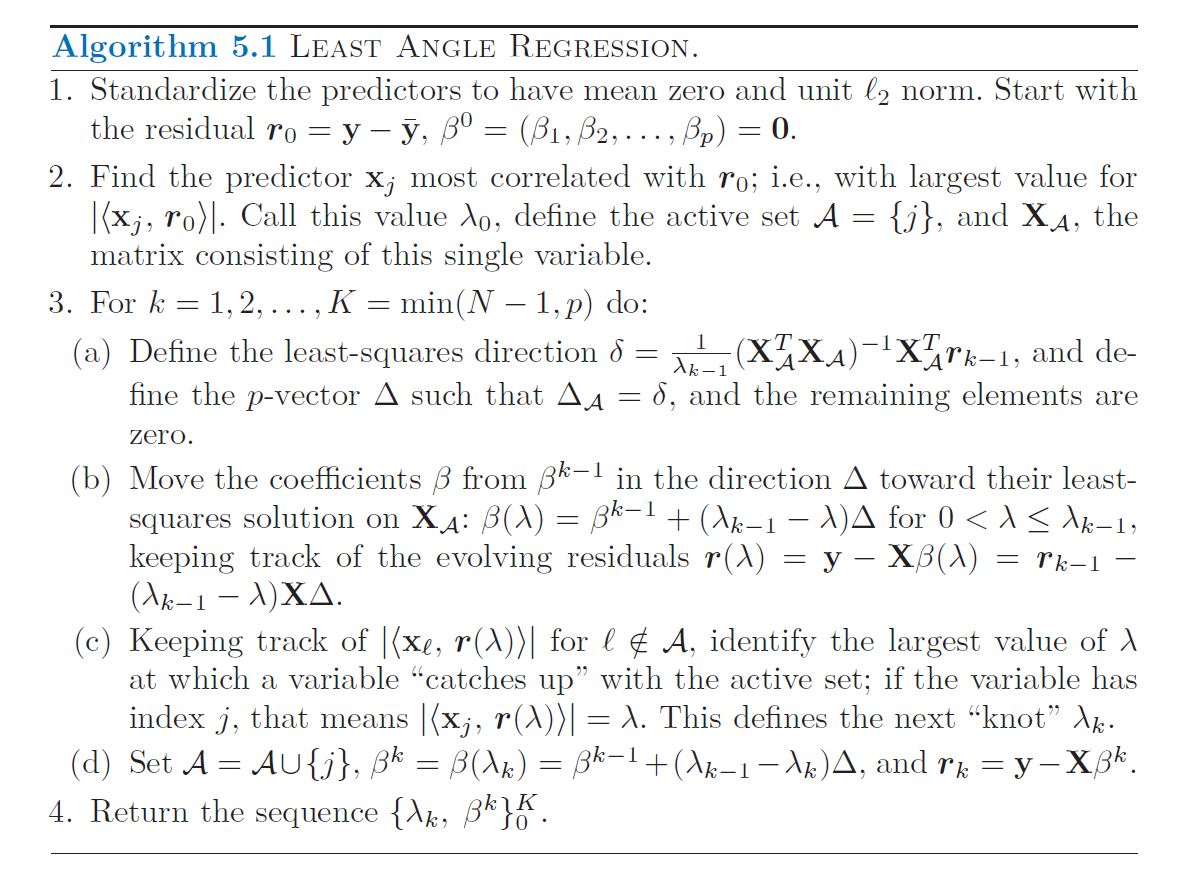
\includegraphics[width=10cm,height=6.5cm]{img/LARS}
\end{figure}
\footnote{Picture taken from \textit{Statistical Learning with Sparsity}  page 119 }
\end{frame}

\begin{frame}{Least Angle Regression: Geometric Representation}
\begin{figure}[h]
\centering
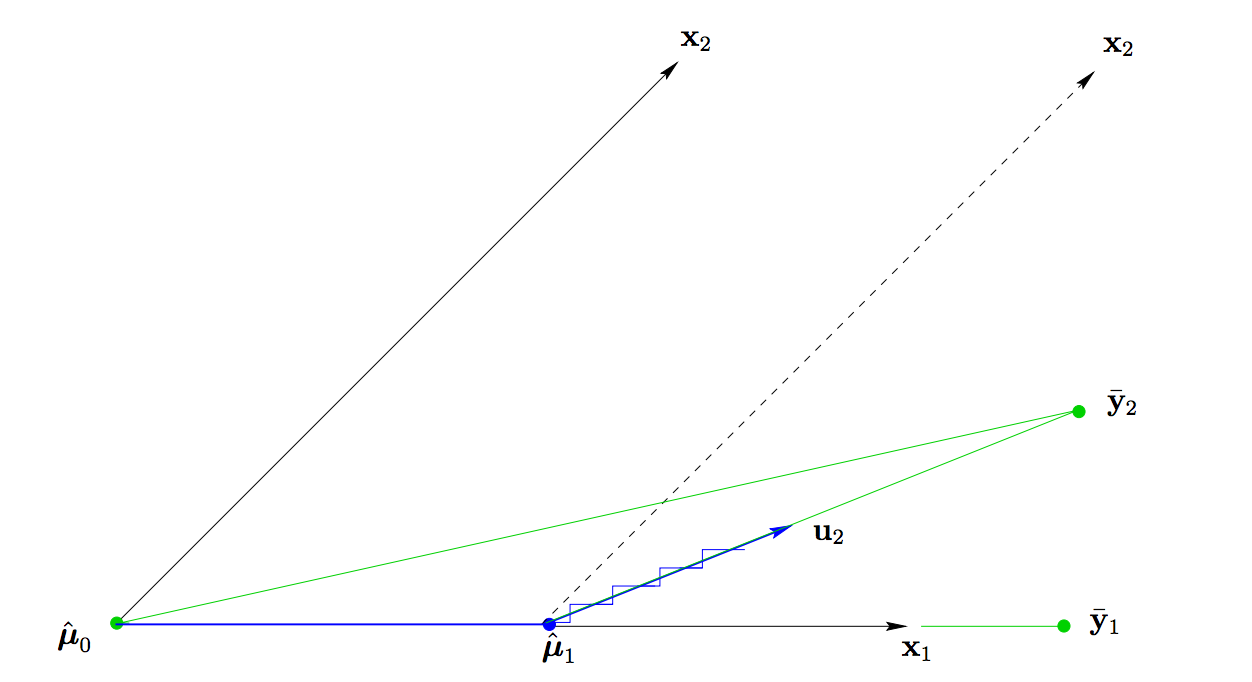
\includegraphics[width=8cm,height=5cm]{img/Geometric}
\end{figure}
\footnote{Figure taken from Efron, Hastie, Johnstore and Tibschirani (2004)}
\note{The LARS algorithm in the case of $m = 2$ covariates; $y_2$ is the projection of $y$ into $L(x1, x2)$. Beginning at $\mu_0 = 0$, the residual vector $y_2 -\mu_0$ has greater correlation with $x_1$ than $x_2$;the next LARS estimate is $\mu_1 =\mu_0 + \gamma_1x_1$, where $\gamma_1$ is chosen such that $y_2 - \mu_1$ bisects the angle
between $x_1$ and $x_2$; then $\mu_2 =\mu_1 + \gamma_2 u_2$, where $u_2$ is the unit bisector; $\mu_2 = y_2$ in the case $m = 2$,but not for the case $m>2$; see Figure 4. The staircase indicates a typical Stagewise path. Here LARS gives the Stagewise track as $\epsilon \to 0$, but a modification is necessary to guarantee agreement in higher dimensions.}
\end{frame}



------------------------------------------------
\section{Comparison of Optimization Methods} %------------------------------------------------
\begin{frame}{Connection between LAR and Lasso}

\begin{block}{LAR}
\vspace*{2mm}
\(\textbf{x}_j^T (\textbf{y}-\textbf{X}\beta(\lambda))=\lambda \cdot s_j,\ 
\forall j \in \mathbb{A}\) \ where \(s_j\) is the sign of inner product \(\lambda\). [3(c)]\\
\end{block} 

\vspace*{3mm}

\only<2>{
\begin{block}{LASSO}
Let \(\mathbb{B}\) be the active set of variables in the solution for a given value of \(\lambda\). \\
\(R(\beta)=\frac{1}{2}\lvert\lvert\textbf{y}-\textbf{X}\beta\rvert\rvert_2^2 + \lambda \lvert\lvert\beta \lvert\lvert_1\) \\
\end{block}
\vspace*{2mm}
For differentiable \(R(\beta)\) , the stationary conditions give: \\
\(\textbf{x}_{j}^{T}  (\textbf{y}-\textbf{X}\beta) =
\lambda \cdot sign(\beta_j), \forall j \in \mathbb{B}\) \\
\vspace*{3mm}
If sign (\(\beta_j\)) matches $s_j$, the coefficient would be identical.

}
\end{frame}

\begin{frame}{Connection between LAR and Lasso}
\begin{itemize}
    \item  R Example
    \vspace*{3mm}
    \item LAR algorithm explains that the coefficient paths for the lasso are \textbf{piecewise linear}
    \vspace*{3mm}
    \item Coefficient paths differ if sign(\(\beta_j\)) is different from $s_j$ 
    \vspace*{3mm}
    
    \item \textbf{Modification} of LAR for computing Lasso solution [3(c)+]: \\
If a \textbf{nonzero} coefficient \textbf{crosses zero} before the next
variable enters, \textbf{drop} it from \(\mathbb{A}\) and recompute the current joint least squares
direction.
    
\end{itemize}
\end{frame}

\begin{frame}{Connection between LAR and Lasso}
\begin{figure}[h]
\centering
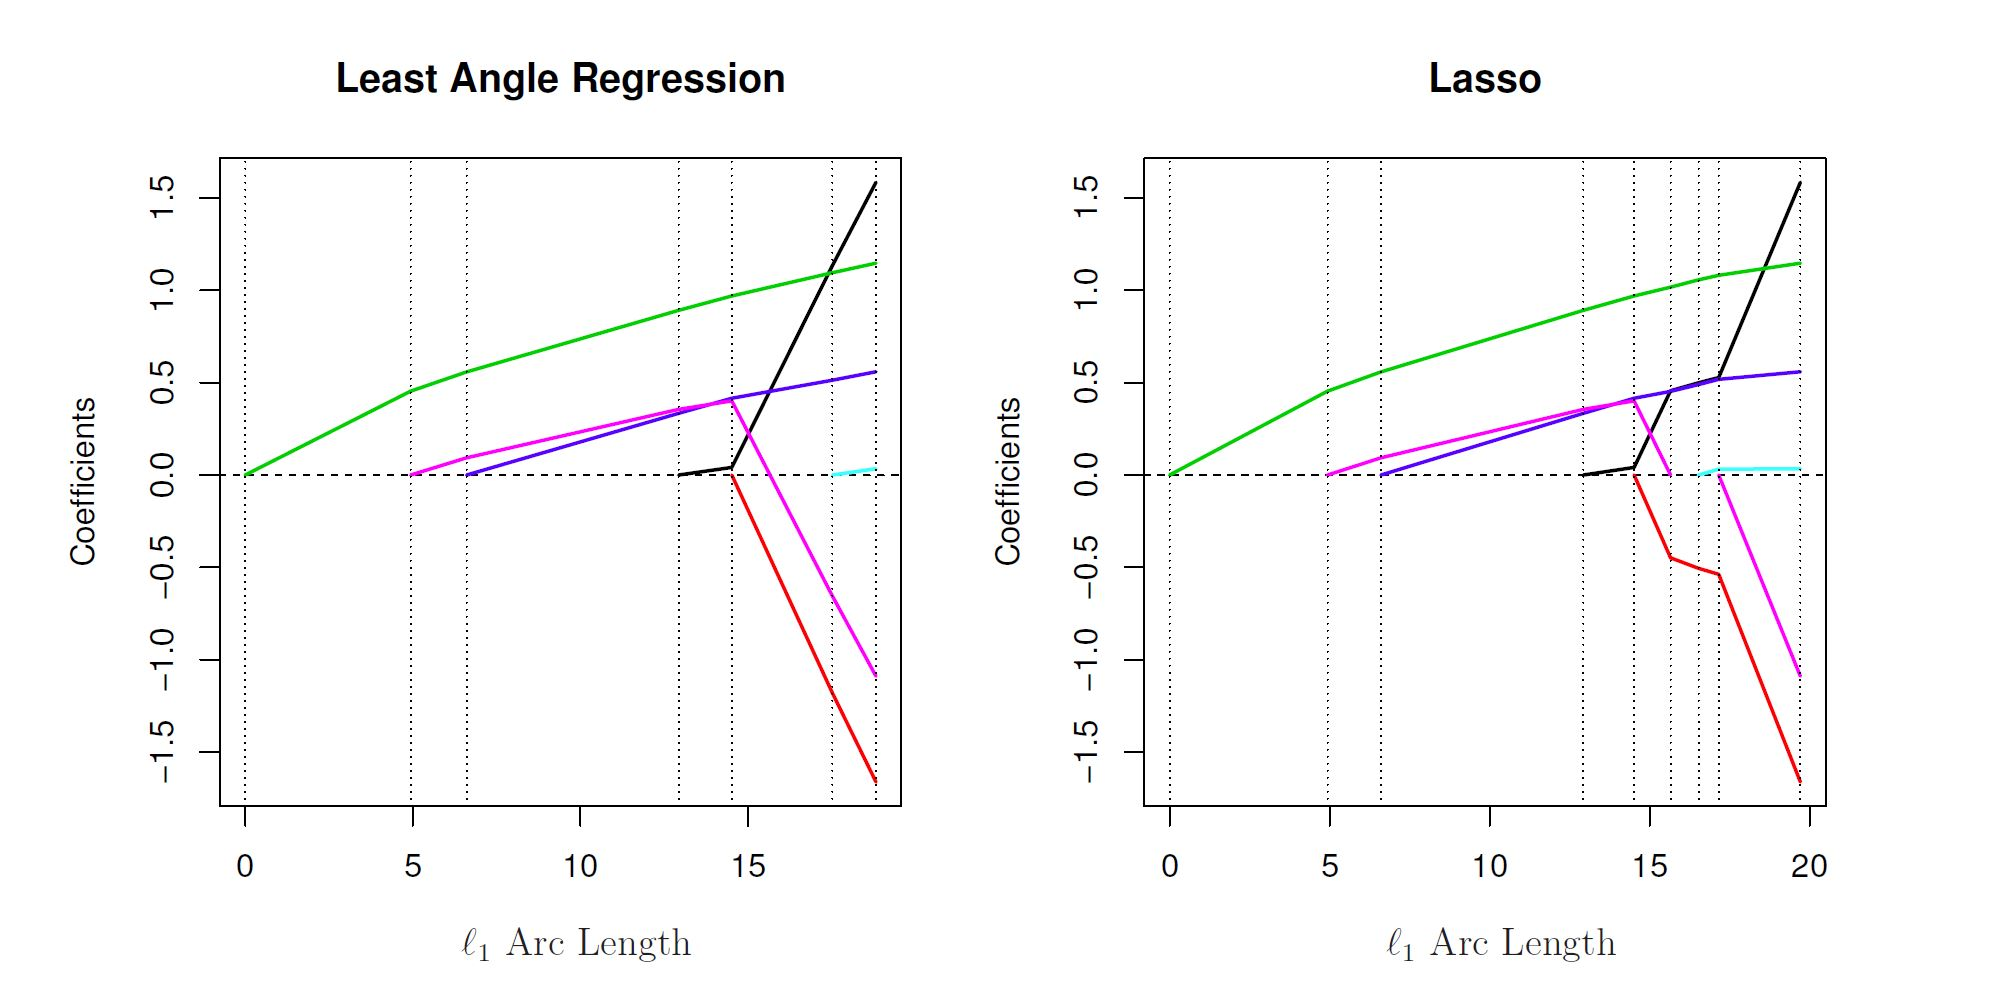
\includegraphics[width=8cm,height=5cm]{img/LARLasso}
\caption{Cases where signs of \(\lambda\) and \(\beta\) disagree}
\end{figure}
\footnote{Picture taken from \textit{Statistical Learning with Sparsity}  page 120 }
\end{frame}

\begin{frame}{Algorithm Performance}
\begin{block} {Simulation: Comparison of computation efficiency between CD and LAR}
\vspace*{3mm}
    Set Up: \footnote{Friedman,Hastie, Tibshirani (2010)}
    \begin{itemize}
        \item Generate Gaussian data with N observations and p predictors, with each pair of predictors \(X_j,X_k\) having the same population correlation \(\rho\).
        \item  Try different combination of $N$ and $p$; Range \(\rho\) from 0 to 0.95.\\
        \(Y=\sum_{j=1}^{p}X_j\beta{j}+kZ\) \ where \( \beta_j= (-1)^j exp(\frac{-2(j-1)}{20}), Z \sim N(0,1)\) and $k$ is a constant.
    \end{itemize}
\end{block}  

\note{Timings (secs) for glmnet and lars algorithms for linear regression with lasso penalty. The first line is glmnet using naive updating while the second uses covariance updating. Total time for 100 \(\lambda\) values, averaged over 3 runs.}
\end{frame}

\begin{frame}{Algorithm Performance}
\begin{figure}[h]
\centering
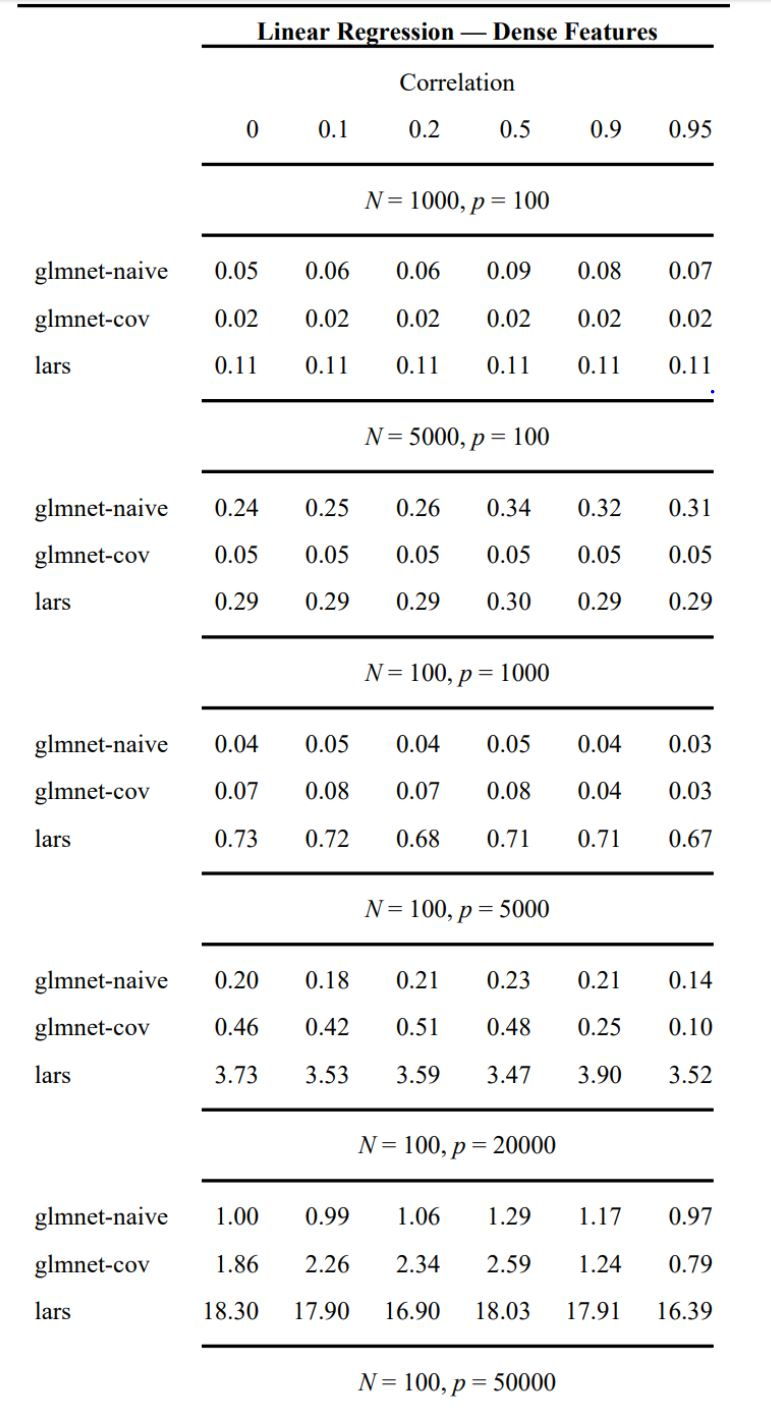
\includegraphics[width=6.5cm,height=7cm]{img/table1}
\caption{Comparison of computing time}
\end{figure}
\footnote{Table taken from the appendix in Friedman,Hastie, Tibshirani (2010) }
\end{frame}

\begin{frame}{Algorithm Performance}
\begin{block}{Simulation: Comparison of computation efficiency between Coordinate Descent, Proximal Gradient Descent and Nestrov Method}
\vspace*{3mm}
Set Up: \footnote{\textit{Statistical Learning with Sparsity} Page 117}
\begin{itemize}
    \item Generated an \(N \times p\) predictor matrix $X$ with standard Gaussian entries and pairwise correlation 0 or 0.5 between the features.
    \vspace*{3mm}
    \item \(\lvert \beta_j \rvert =exp \big[ -0.5(u(j-1))^2\big] \) and \ 
    \(u=\sqrt{\frac{\pi}{20}}\) and alternating signs -1,+1,-1...
\end{itemize}
\end{block}
\end{frame}

\begin{frame}{Algorithm Performance}
\begin{figure}[h]
\centering
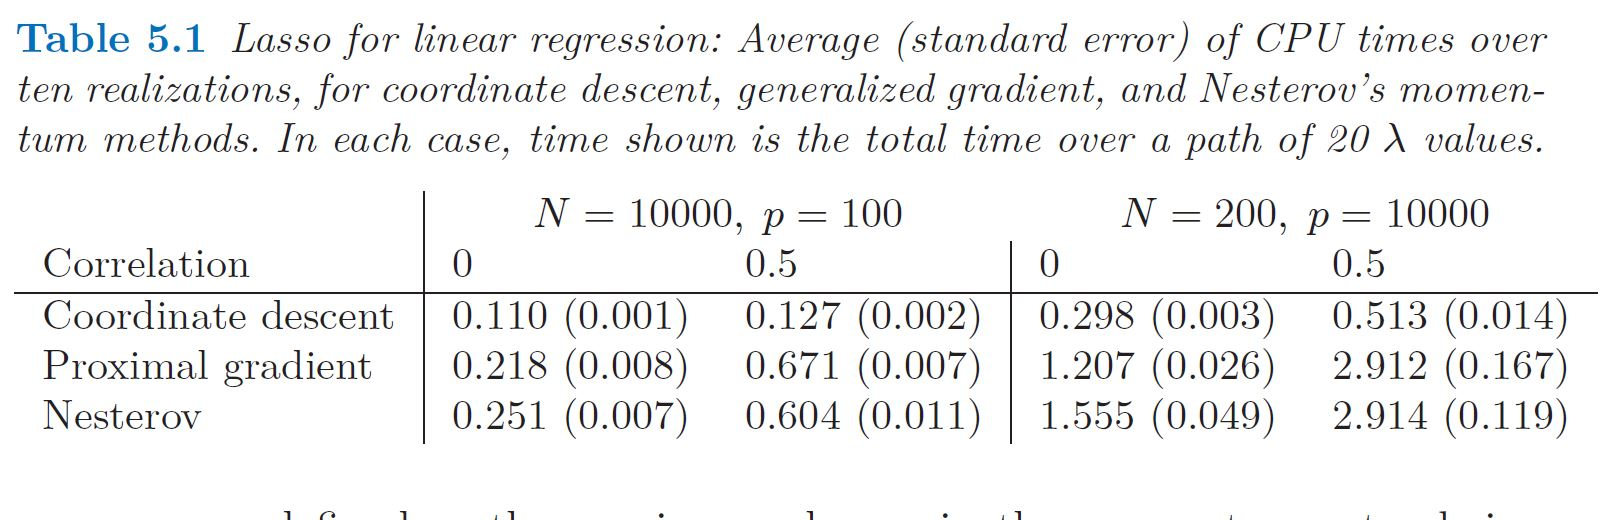
\includegraphics[width=7cm,height=3cm]{img/table2}
\caption{Comparison of computing efficiency between 3 methods}
\end{figure}
 \footnote{\textit{Statistical Learning with Sparsity} Page 117}  
\end{frame}



%------------------------------------------------
\section{Recall: Duality}
%------------------------------------------------

\begin{frame}
\frametitle{Recall: Duality in optimization}

%\begin{tabular}{lcc}
%\toprule
%&Primal&Dual\\\midrule
%Optimize&$\min f(x)$&$\max q(\lambda,\mu)$\\\midrule
%Constraints&$g_i(x)\le0, h_j(x)=0, x\in X$&$\lambda\ge0$\\\midrule
%Function&$L(x,\lambda,\mu):=f(x)+\sum_i\lambda_i g_i(x)+\sum_j\mu_j h_j(x)$&$q(\lambda,\mu)=\inf\limits_{x\in X} L(x,\lambda,\mu)$\\
%&$L(x,\lambda,\mu):=f(x)+\lambda^Tg(x)+\mu^T h(x)$&\\\midrule
%\end{tabular}



%\vspace{15pt}
%Why though? - \textbf{Dual problem is always convex!}

\end{frame}
\note{In various section, I came across terms like "dual" and "dual problem"}

\begin{frame}
\begin{tabular}{ll}
\toprule[1.5pt]
\multicolumn{2}{c}{Primal}\\\midrule
Optimize&$\min f(x)$\\\midrule
Constraints&$g_i(x)\le0, h_j(x)=0, x\in X$\\\midrule
Function&$L(x,\lambda,\mu):=f(x)+\sum_i\lambda_i g_i(x)+\sum_j\mu_j h_j(x)$\\\midrule
%&$L(x,\lambda,\mu):=f(x)+\lambda^Tg(x)+\mu^T h(x)$\\\midrule
\multicolumn{2}{c}{Dual}\\\midrule
Function&$q(\lambda,\mu)=\inf\limits_{x\in X} L(x,\lambda,\mu)$\\\midrule
Constraints&$\lambda\ge0$\\\midrule
Optimize&$\max\limits_{\lambda\ge0,\mu} q(\lambda,\mu)$\\\midrule
\end{tabular}
\vspace{15pt}

Why though? - \textbf{Dual problem is always convex!}

\end{frame}

\note{
$x\in X$ for e.g. solutions in a cone or integer solutions

%$g$ and $h$ are now in vector notation

Terms: Primal problem, Lagrange function with dual variables/Lagrange-multipliers, dual function ($\lambda$ and $\mu$ now in vector notation), dual problem (max q)


Dual problem is always convex! - I don't know much about optimization yet, but
they really like convexity.

"(Convexity confers two advantages. The first is that, in a constrained problem, a convex feasible region makes it easier to ensure that you do not generate infeasible solutions while searching for an optimum.)

The second advantage is that all local optima are global optima. That allows local search algorithms to guarantee optimal solutions. And local search is often faster." \cite{ru16})



}



%------------------------------------------------
\section{ADMM}
%------------------------------------------------

\begin{frame}
\frametitle{Alternating Direction Method of Multipliers (ADMM)}
Problem\only<2->{ - decomposable ! }
\only<2>{\note{decomposable problem and constraints!}
}
\[\underset{\beta\in\R^m, \theta\in\R^n}{\text{minimize}}f(\beta)+g(\theta)\quad\text{subject to}\ \mathbf{A}\beta+\mathbf{B}\theta-c=0\]
%\note{decomposable problem and constraints!\\}
Lagrangian\only<3->{ - decomposable !}
\only<3>{\note{Lagrangian problem can still be decomposed into $\beta$ and $\mu$ terms

this has nice algorithm where we can execute some stuff in parallel, because we can decompose the Lagrangian}
}
\[f(\beta)+g(\theta)+\left\langle\mu,\mathbf{A}\beta+\mathbf{B}\theta-c\right\rangle\]
Augmented Lagrangian\only<4->{ - NOT decomposable !}
\only<4>{
\note{
Augmented: scalar product with $\rho$ gets added, 

Method of Multipliers: is a way to make the algorithm more robust 

advantage: better convergence

disadvantage: no longer parallel execution of subtasks due to l2-term, no longer decomposable in beta and theta terms, as l2 norm dquares every entry of the vector

alternating direction: semi-decomposable, i.e. keeping one variable fixed while updating the other

$\rho$ is step length of iterative algorithm

All notes on this slide: see the slides by \cite{boyd}

}
}
\[L_{\rho}(\beta,\theta,\mu):=f(\beta)+g(\theta)+\left\langle\mu,\mathbf{A}\beta+\mathbf{B}\theta-c\right\rangle+\frac{\rho}{2}||\mathbf{A}\beta+\mathbf{B}\theta-c||_2^2\]
\end{frame}



\begin{frame}
\frametitle{Dual Variable Update}
\framesubtitle{Alternating Direction Method of Multipliers}
\begin{align*}
\beta^{t+1}&=\argmin_{\beta\in\R^m}L_{\rho}(\beta,\theta^t,\mu^t)\\
\theta^{t+1}&=\argmin_{\theta\in\R^m}L_{\rho}(\beta^{t+1},\theta,\mu^t)\\
\mu^{t+1}&=\mu^t+\rho(\mathbf{A}\beta^{t+1}+\mathbf{B}\theta^{t+1}-c)
\end{align*}
\pause
%\only<2>{
\visible<2>{
\begin{figure}
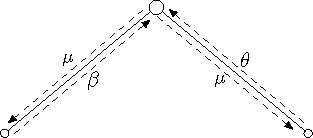
\includegraphics{img/dualascentstep.pdf}
\caption{My own illustration of the dual ascent step in the ADMM algorithm utilising dual decomposition based on \cite{GT12}.}
\end{figure}
}
%}

\end{frame}

\note{
Method of Multipliers: is a way to make the algorithm more robust, (if in second line $\beta^t$ statt $\beta^{t+1}$)

alternating direction: semi-decomposable, i.e. keeping one variable fixed while updating the other

think of it as only the last line, sending $\mu$ to the updaters for $\beta$ and $\theta$

in this context $\rho$ in last line can be thought of as "step length"

All notes on this slide: see the slides by \cite{boyd}
}

\begin{frame}
\frametitle{ADMM - Why?}
\begin{itemize}
\item[-] convex problems with nondifferentiable constraints
\item[-] blockwise computation
	\begin{itemize}
	\item[-] sample blocks
	\item[-] feature blocks
	\end{itemize}
\end{itemize}
\end{frame}

\note{
Details for blockwise computation in Exercise 5.12.
}

\begin{frame}
\frametitle{ADMM for the Lasso}
\framesubtitle{Problem}
Problem in Lagrangian form
\[\underset{\beta\in\R^p,\theta\in\R^p}{\text{minimize}}\left\{\frac{1}{2}\Norm{\mathbf{y}-\mathbf{X}\beta}_2^2+\lambda\Norm{\theta}_1\right\}\quad \text{such that}\ \beta-\theta=0 \]
\vspace{15pt}

Augmented Lagrangian
\[L_{\rho}(\beta,\theta,\mu):=\left\{\frac{1}{2}\Norm{\mathbf{y}-\mathbf{X}\beta}_2^2+\lambda\Norm{\theta}_1\right\}+\left\langle\mu,\beta-\theta\right\rangle+\frac{\rho}{2}||\beta-\theta||_2^2 \]
\end{frame}

\note{
In the problem, I can decompose into beta and theta terms, i.e.show $f(\beta)$ and $g(\theta)$

the problem itself and the constraints, 

A and B are unit matrices here

}


\begin{frame}
\frametitle{ADMM for the Lasso}
\framesubtitle{Update}
Update
\begin{align*}
\beta^{t+1}&=(\mathbf{X}^T\mathbf{X}+\rho\mathbf{I})^{-1}(\mathbf{X}^T\mathbf{y}+\rho\theta^t-\mu^t)\\
\theta^{t+1}&=\mathcal{S}_{\lambda/\rho}(\beta^{t+1}+\mu^t/\rho)\\
\mu^{t+1}&=\mu^t+\rho(\beta^{t+1}-\theta^{t+1})
\end{align*}
where $\mathcal{S}_{\lambda/\rho}(z)=\text{sign}(z)(\norm{z}-\frac{\lambda}{\rho})_+$.

\end{frame}

\note{
$\mathcal{S}$ is a soft-thresholding parameter

Computational cost: Initially $\mathcal{O}(p^3)$, which is a lot, for the SVD(singular value decomposition of $\mathbf{X}$), after that comparable to coordinate descent or composite gradient from earlier
}


%------------------------------------------------
\section{Screening Rules}
%------------------------------------------------

\begin{frame}
\frametitle{Screening Rules}

\begin{itemize}
	\item[-] Pre-processing to eliminate features
	\item[-] very big data set, esp. huge number of predictors
	\item[-] maybe too big to load into memory
	\item[-] Screening rules eliminate predictors with minor calculation
	\item[-] and very high / safe certainty (i.e. eliminated predictors would not show up in lasso model based on full data)
\end{itemize}


They achieve a reduction in the number of variables, typically by an order of magnitude

\note{Imagine a big data set, a very big data set, with such a huge design matrix, that you cannot load it into memory (RAM).}

% add stuff from notes


\end{frame}

\begin{frame}
\frametitle{What is a good predictor?}

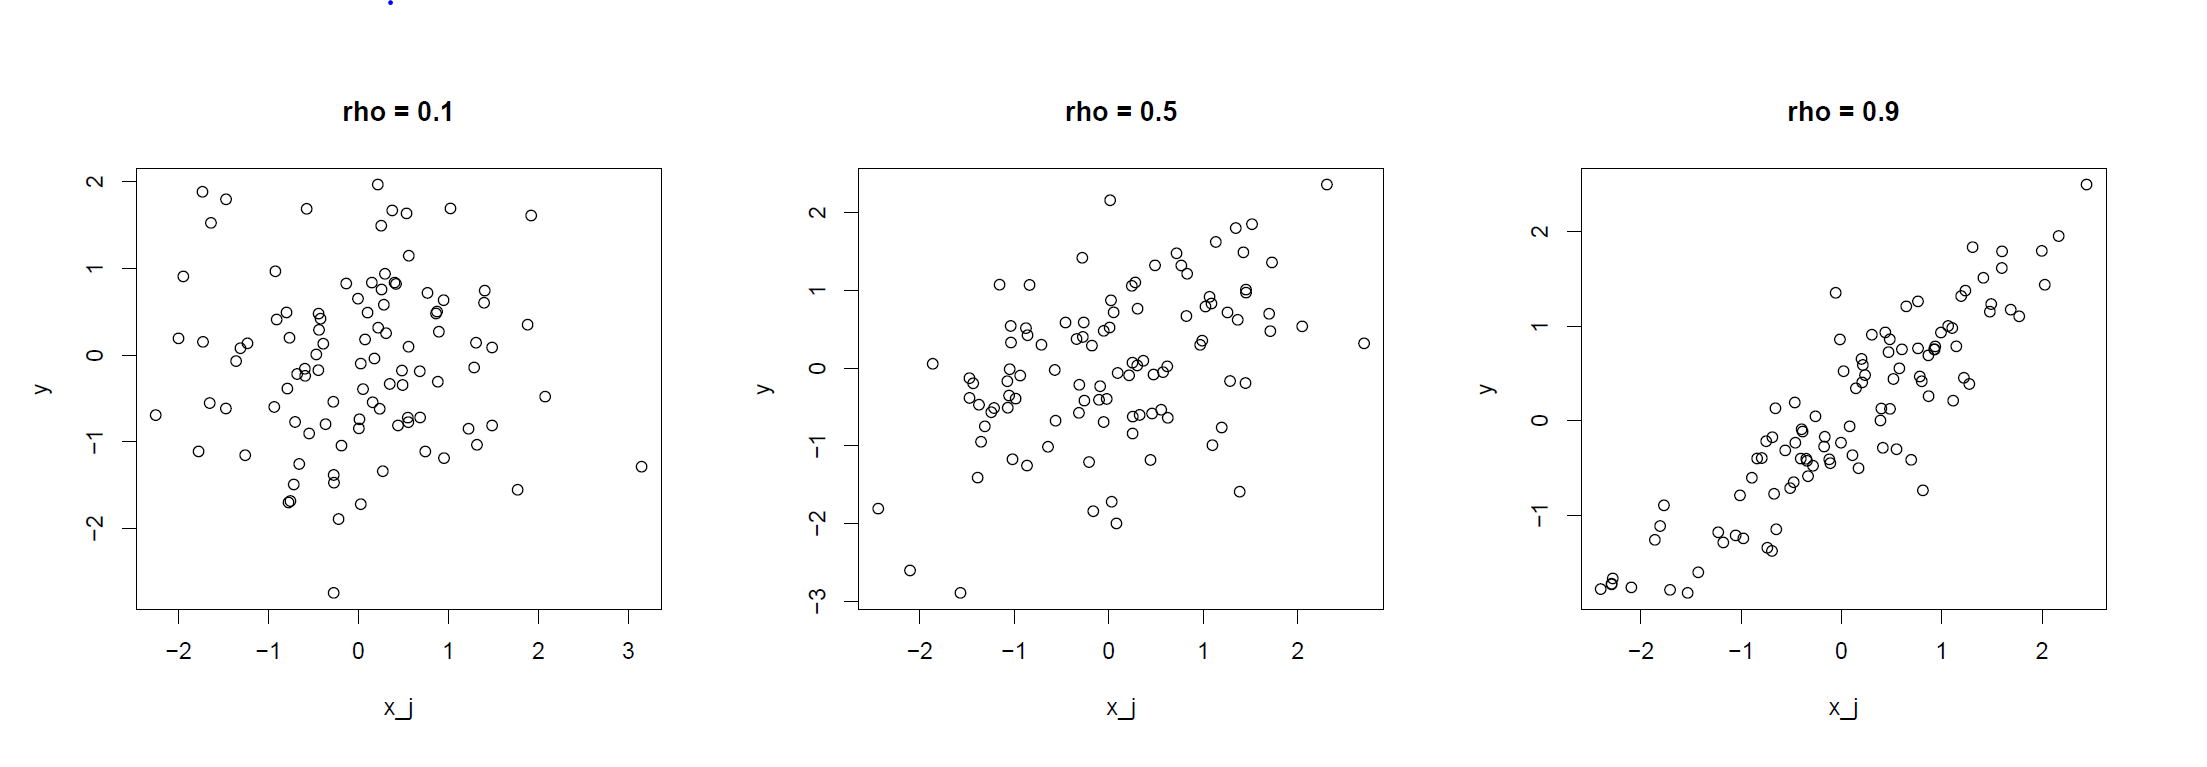
\includegraphics[width=\linewidth]{img/differentCorrelationPlots}

correlation is an inner product

high absolute correlation (=large absolute inner product) 

$->$ high predictive power (compare plots) 

$->$ $x_j$ with largest inner product has highest predictive power, thus for that j we are most willing to accept some penalty from $\lambda$

\end{frame}

\begin{frame}
\frametitle{Lasso - an iterative algorithm}
Let $\mathcal{A}$ be the active set of predictors. Let $\lambda$ take values on a decreasing sequence.

\vspace{15pt}

iterate

\begin{enumerate}
	\item order predictors $x_j$ not in $\mathcal{A}$ by their "effectiveness" using $\norm{x_j^Ty}$ or better $\norm{x_j^T(y-\hat{y}_{\lambda})}$, call the best predictor $x_{j_{\max}}$
	\item move $\lambda$ such that the positive effect from the best predictor $x_{j_{\max}}$ compensates the penalty by $\lambda$
	\item calculate solution for chosen $\lambda$
\end{enumerate}

\end{frame}

\note{
this is just a formalisation of the previous slide

or better b/c we want to focus on the residuals once we have a preliminary solution
}

\begin{frame}
\frametitle{Lasso - a visual intepretation}

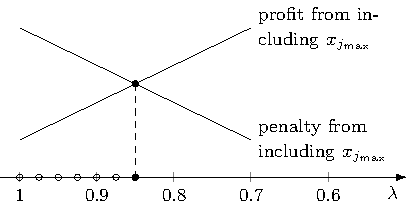
\includegraphics[width=\linewidth]{img/lassodifferentperspective.pdf}

\note{
visualisation of step 2 of the previous slide

these lines are not linear, neither is usually the spacing on the lambda axis

we are walking along the lambda axis until we find a good point / the intersection between the penalty and the profit}
\end{frame}

\begin{frame}
\frametitle{Back to screening rules}
Let $\lambda$ take values on a decreasing sequence. Let $\lambda_{\max}$ be the $\lambda$ where the first predictor has a non-zero coefficient.
\[\lambda_{\max}=\max_j\norm{x_j^Ty}\]
Let $\mathcal{A}$ be the active set of predictors.
\[\forall j \in\mathcal{A}\ \ \lambda=\norm{x_j^T(y-\hat y)}\]

\only<1>{\[\forall j \notin\mathcal{A}\ \ \lambda\ge\norm{x_j^T(y-\hat y)}\]

\note{
for those wondering why in first equation not y-yhat? anybody?

yhat would come from the empty/intercept model, i.e. yhat=mean(y)

we assume standardised data (i.e. mean 0 and unit variance)

thus yhat = 0
}
}
\only<2>{
\vspace{5pt}

{\centering\colorbox{red!40}{$\forall j \notin\mathcal{A}\ \ \lambda\ge\norm{x_j^T(y-\hat y)}$}

\vspace{10pt}}

R example

\note{
this is the essential equation for screening rules, if, for a given lambda, a predictor does not fulfil this equation, we kick it out

\textbf{SHOW R STUFF SCREENINGRULES 2}
}
}

\end{frame}

\begin{frame}
\frametitle{Global vs. Sequential}


Global (one-time screening): 

Suppose we want to calculate a lasso solution at $\lambda<\lambda_{\max}$. 

\vspace{25pt}
Sequential (iterative screening): 

Suppose we have the lasso solution $\hat\beta(\lambda')$ at $\lambda'$ and want to screen variables for solutions at $\lambda<\lambda'$.

\end{frame}

\note{There are two main classes of Screening rules}

%\begin{frame}
%\frametitle{SAFE Rules}
%
%
%\end{frame}

\begin{frame}
\frametitle{Dual Polytope Projection (DPP)}
Suppose we want to calculate a lasso solution at $\lambda<\lambda_{\max}$. The DPP rule discards the $j^{th}$ variable if 
\[\norm{\mathbf{x}_j^T\mathbf{y}}<\lambda_{\max}-\Norm{\mathbf{x}_j}_2\Norm{\mathbf{y}}_2\frac{\lambda_{\max}-\lambda}{\lambda}\]

\vspace{5pt}
{\hspace{5pt}\Large Sequential DPP rule}
\vspace{15pt}

Suppose we have the lasso solution $\hat\beta(\lambda')$ at $\lambda'$ and want to screen variables for solutions at $\lambda<\lambda'$. We discard the $j^{th}$ variable if 
\[\norm{\mathbf{x}_j^T(\mathbf{y}-\mathbf{X}\hat{\beta}(\lambda'))}<\lambda'-\Norm{\mathbf{x}_j}_2\Norm{\mathbf{y}}_2\frac{\lambda_{\max}-\lambda}{\lambda}\]
\end{frame}

\begin{frame}
\frametitle{Global Strong Rule}
Suppose we want to calculate a lasso solution at $\lambda<\lambda_{\max}$. The global strong rule discards the $j^{th}$ variable if 
\[\norm{\mathbf{x}_j^T\mathbf{y}}<\lambda-(\lambda_{\max}-\lambda)=2\lambda-\lambda_{\max}\]

\vspace{5pt}
{\hspace{5pt}\Large Sequential Strong Rule}
\vspace{15pt}

Suppose we have the lasso solution $\hat\beta(\lambda')$ at $\lambda'$ and want to screen variables for solutions at $\lambda<\lambda'$. We discard the $j^{th}$ variable if 
\[\norm{\mathbf{x}_j^T(\mathbf{y}-\mathbf{X}\hat{\beta}(\lambda'))}<2\lambda-\lambda'\]
\end{frame}

\begin{frame}
\frametitle{Screening Rules - Example Setup}

\begin{itemize}
	\item simulated dataset
	\item $N = 200, p = 5000$ uncorrelated Gaussian predictors, 
	\item $1/4$ true non-zero coefficients 
	\item 100 decreassing lambda values equally spaced on the log-scale
	\item Compare Global DPP, Global Strong, Sequential DDP, Sequential Strong
	\item no violations for either of the strong rules
\end{itemize}

\end{frame}

\begin{frame}
\begin{figure}

\caption{From \cite{Has15}}
\end{figure}
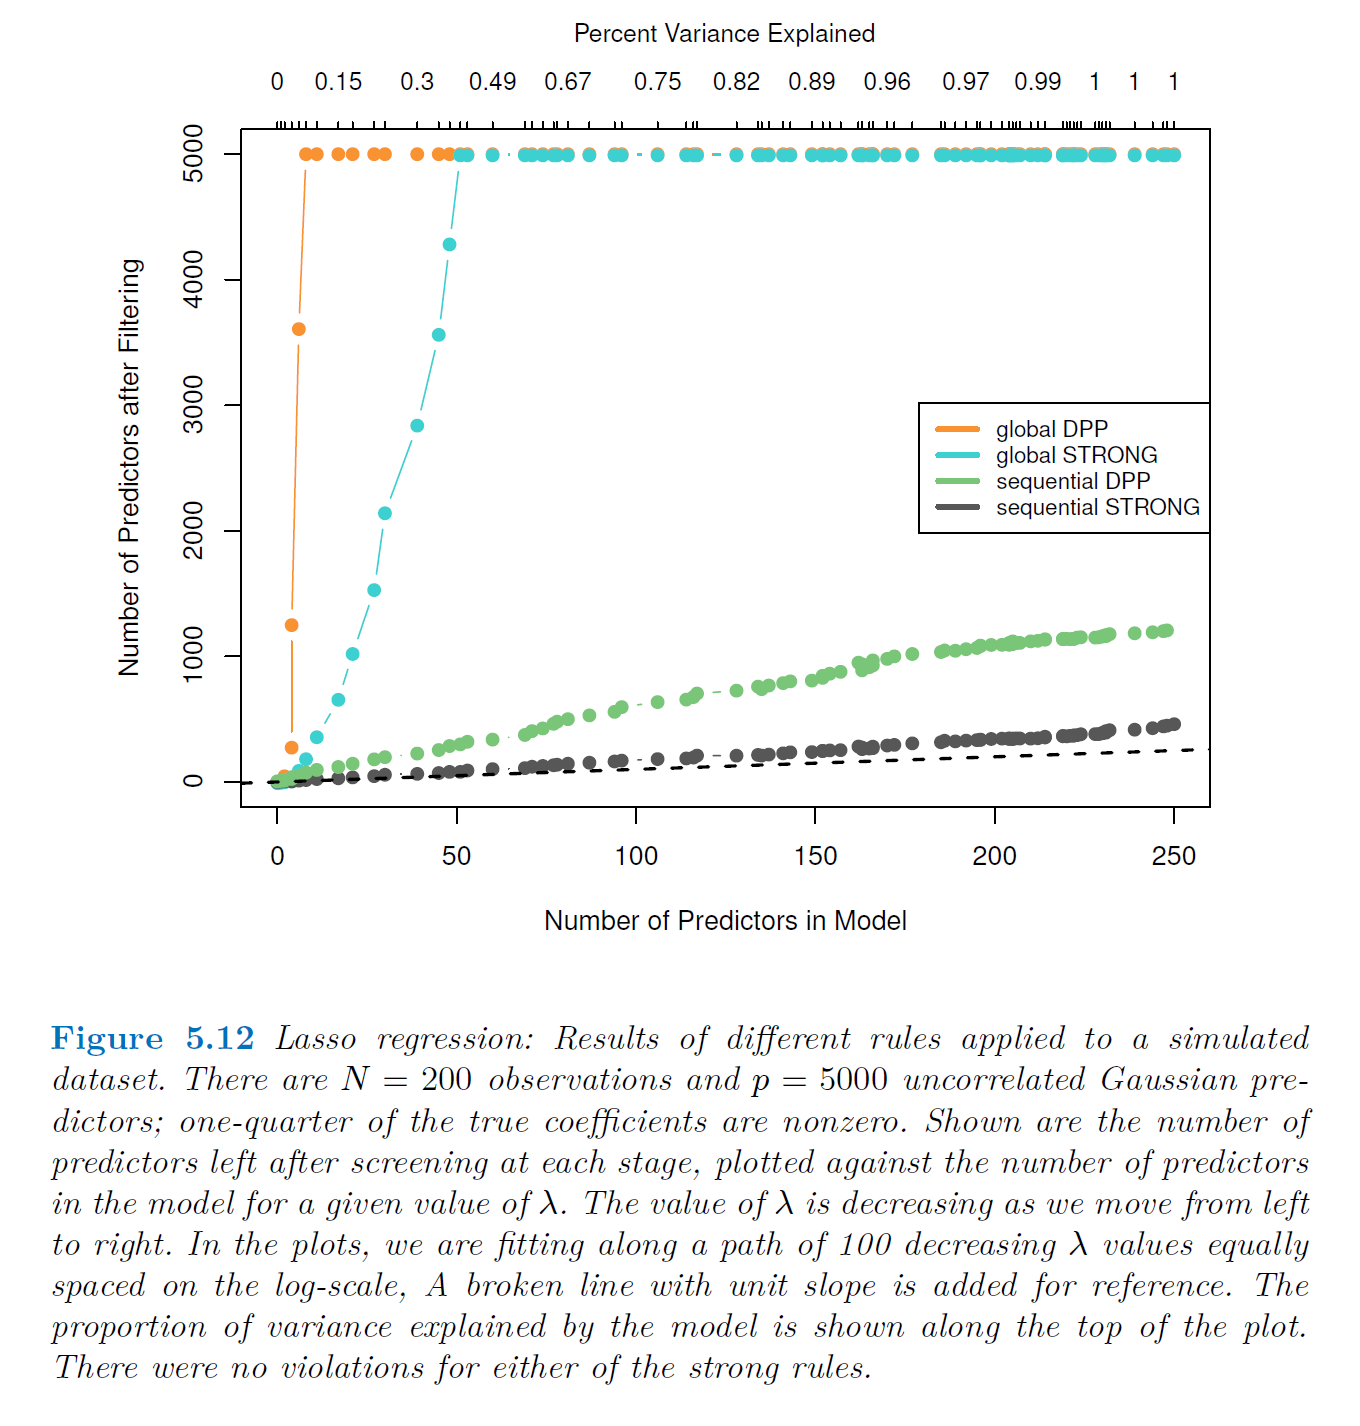
\includegraphics[width=\linewidth]{img/screeningrulesoverview.png}
\end{frame}

\note{
Lasso regression: Results of different rules applied to a simulated
dataset. There are N = 200 observations and p = 5000 uncorrelated Gaussian predictors; one-quarter of the true coefficients are nonzero. Shown are the number of predictors left after screening at each stage, plotted against the number of predictors in the model for a given value of $\lambda$. The value of  $\lambda$ is decreasing as we move from left  to right. In the plots, we are fitting along a path of 100 decreasing $\lambda$ values equally spaced on the log-scale, \textbf{A broken line with unit slope is added for reference.} The proportion of variance explained by the model is shown along the top of the plot. There were no violations for either of the strong rules.
}

\begin{frame}{Summary I}
\begin{block}{Coordinate Descent}
\begin{itemize}
    \item An efficient algorithm implemented in glmnet but requires separability condition
    \item Application: Ridge, Lasso, Elastic Net, Logistic Regression, etc.
\end{itemize}
\begin{block}{Least Angle Regression }
\begin{itemize}
    \item Similar to the idea of Forward Selection 
    \item Computationally efficient but does not scale well to large problems
\end{itemize}
\begin{block}{Connection between LASSO and LAR}
\begin{itemize}
    \item LAR could be modified to obtain Lasso solution 
    \item Explains the fact that Lasso coefficient solution path is piece-wise linear
\end{itemize}

\end{block}

\end{block}

\end{block}
\end{frame}

\begin{frame}
\frametitle{Summary II}
\begin{block}{ADMM}
\begin{itemize}
	\item Use duality to your advantage
	\item Limitations in speed for Lasso, but useful in more complex settings
\end{itemize}
\begin{block}{Screening Rules}
\begin{itemize}
    \item Promising for very large $p$'s 
    \item Difficult to find best rule, field in development
\end{itemize}


\end{block}


\end{block}

\end{frame}

%------------------------------------------------
\section{Minor-Max Algorithms}
%------------------------------------------------

\begin{frame}
\frametitle{Minorization-Maximization Algorithms (MMA)}
\begin{itemize}
\item[-] Problem: minimize $f(\beta)$ over $\beta\in\R^p$\\ for $f$ possibly non-convex
\item[-] Introduce additional variable $\theta$
\item[-] Use $\theta$ to majorize (bound from above) the objective function to be minimized
\end{itemize}


{\small Majorization-Minimization Algorithms work analoguosly.}
\end{frame}

\begin{frame}
\frametitle{MMA visually}
\begin{figure}
%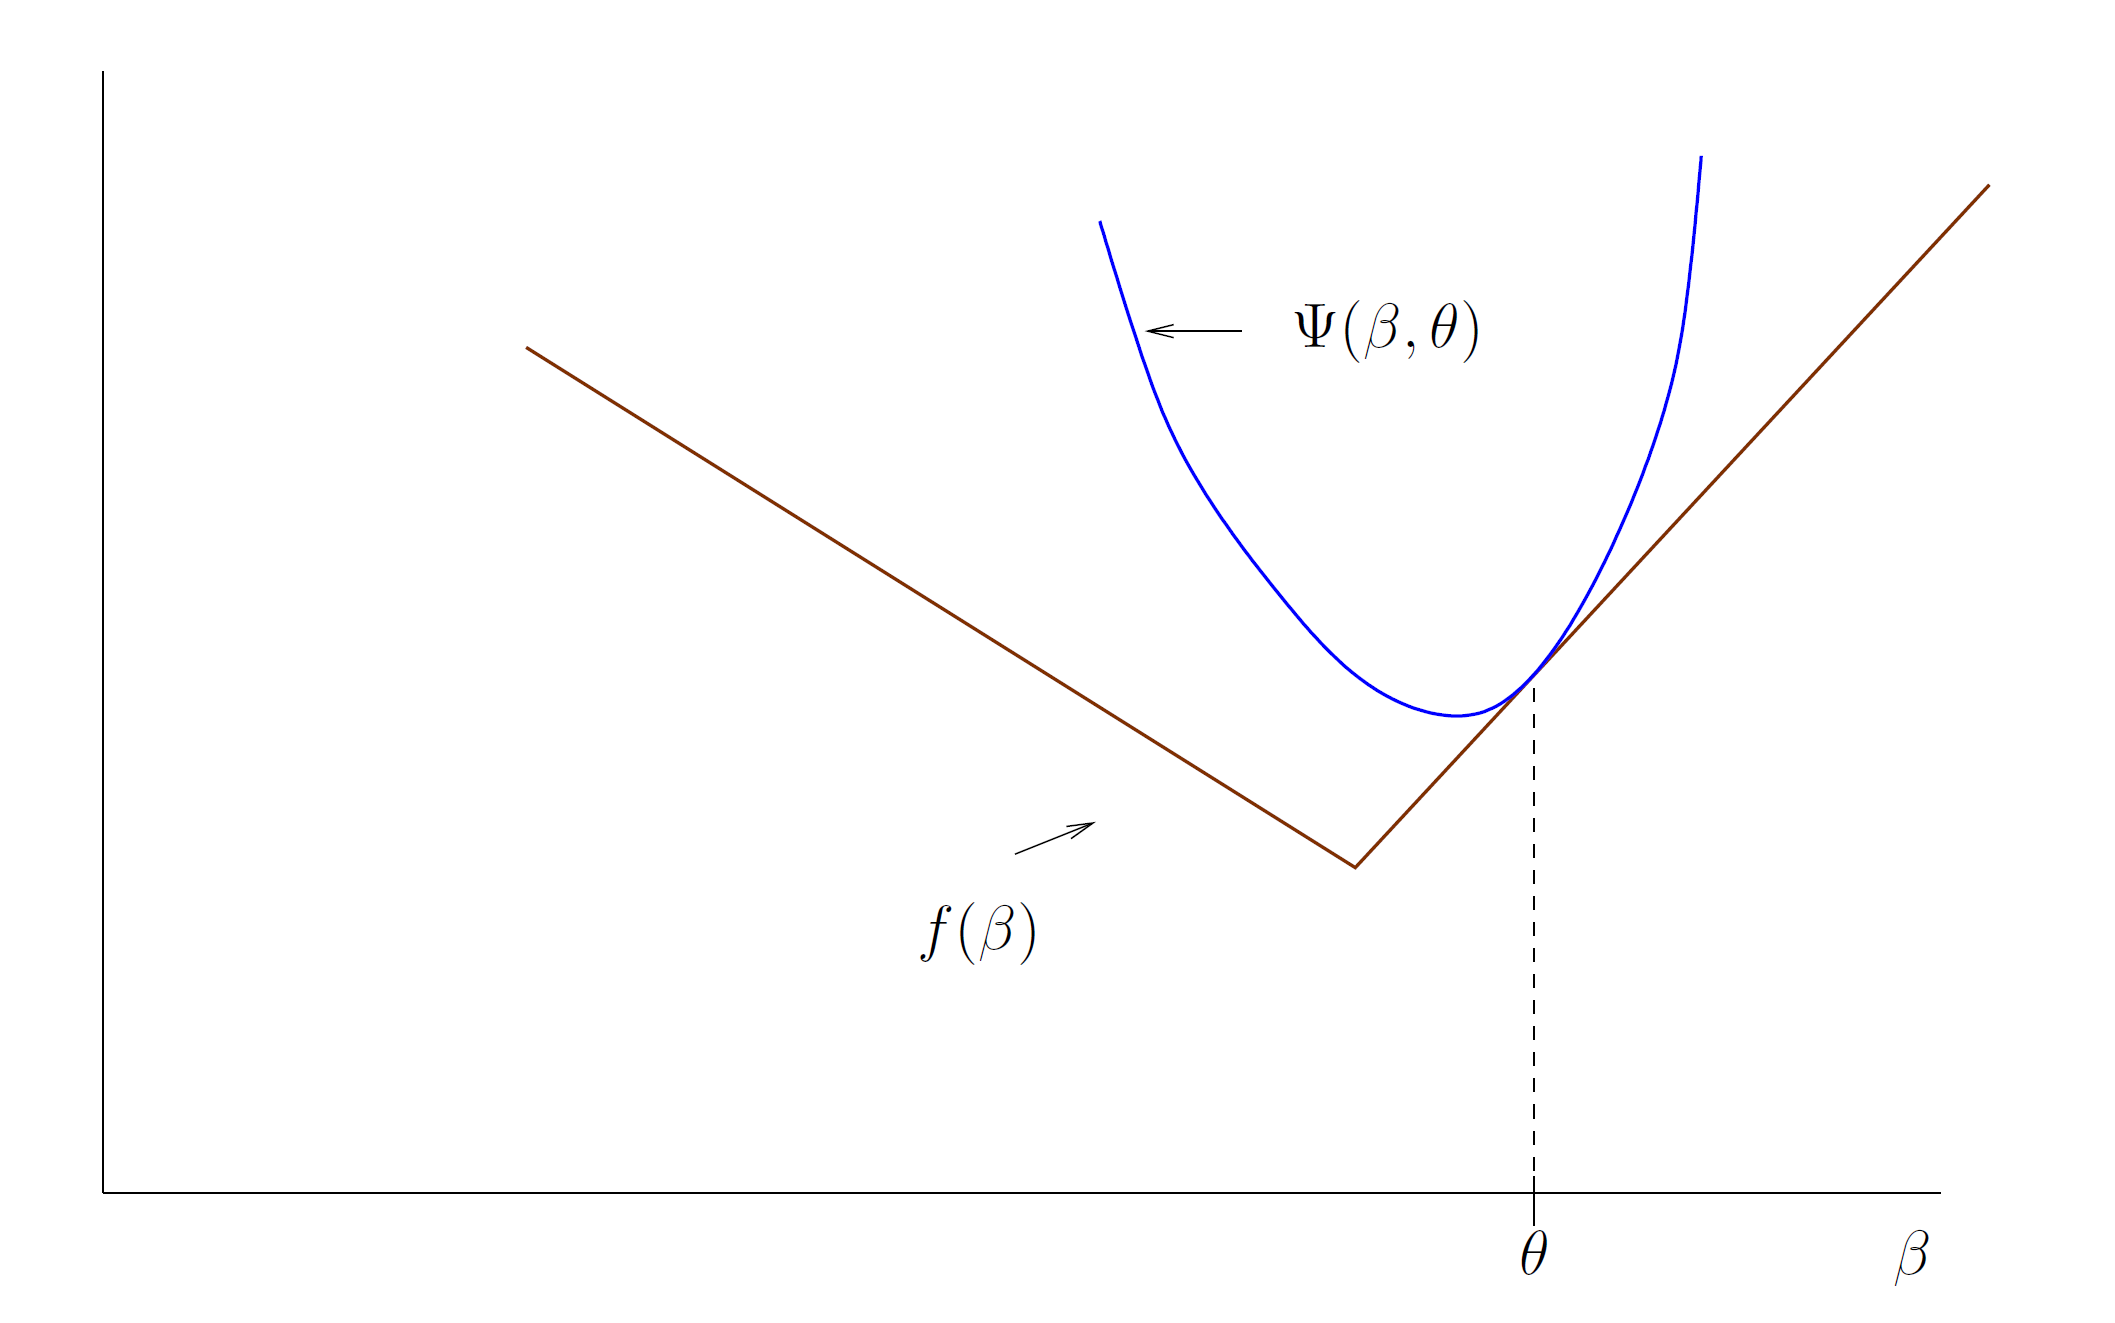
\includegraphics[width=\textwidth]{img/minmaxalgo.png}
%\caption{Figure 5.10 from \cite{Has15}}
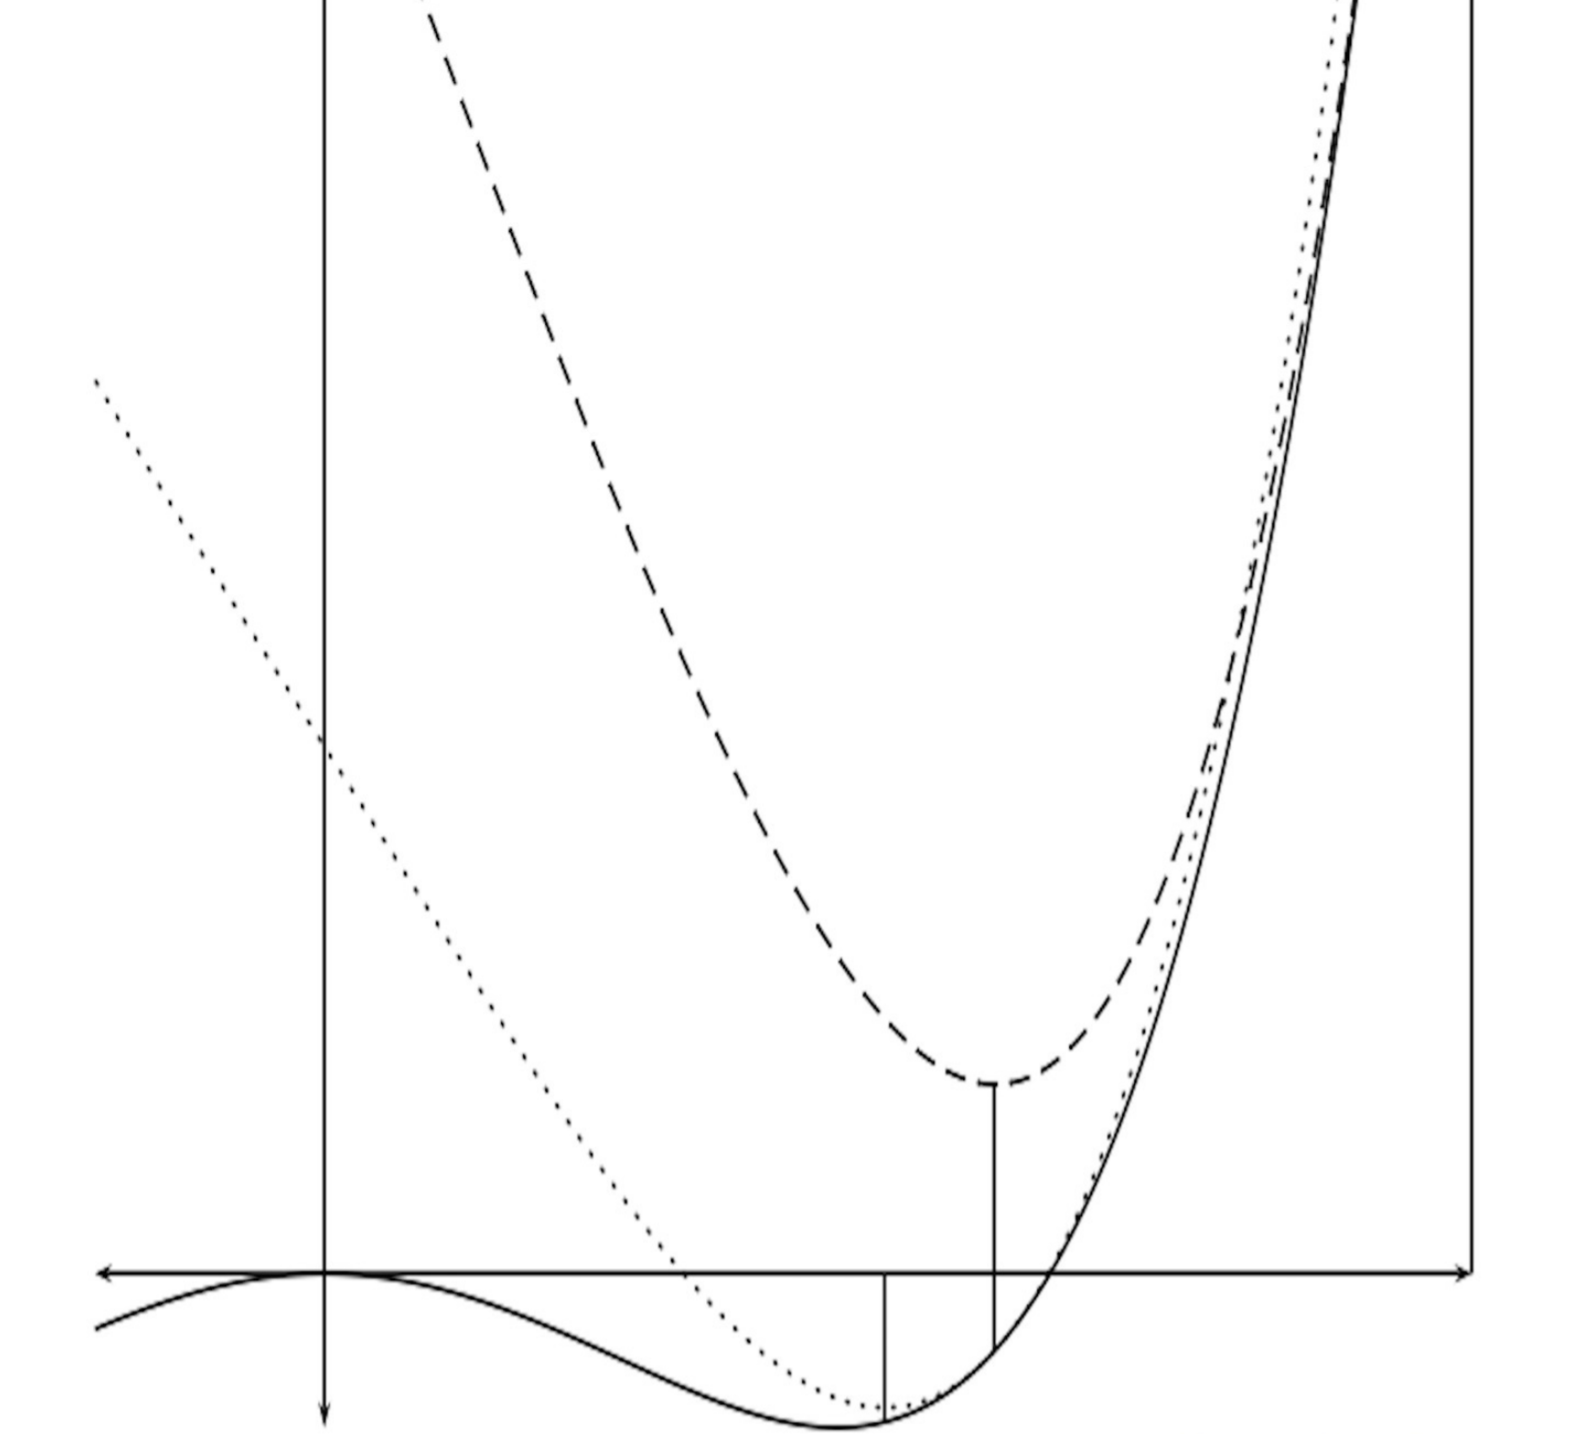
\includegraphics[height=150pt]{img/minmaxalgo2.png}
\caption{Figure from \cite{DL15}}
\end{figure}

\end{frame}

\begin{frame}
\frametitle{MMA analytically I}
Def. 
$\Psi:\R^p\times\R^p\to\R$ {\color{blue}majorizes} $f$ at $\beta\in\R^p$ if \[\forall\theta\in\R^p\quad \Psi(\beta,\theta)\ge f(\beta)\]
with equality for $\theta=\beta$.
\vspace{10pt}

Minor-Maxxalgorithm
\begin{itemize}
\item[-] initialize $\beta^0$
\item[-] update with $\beta^{t+1}=\argmin\limits_{\beta\in\R^p}\Psi(\beta,\beta^t)$
\end{itemize}
\end{frame}

\begin{frame}
\frametitle{MMA analytically II}
This scheme generates a sequence of $\beta$'s for which the cost $f(\beta^t)$ is nonincreasing, because
\[f(\beta^t)\stackrel{(i)}{=}\Psi(\beta^t,\beta^t)\stackrel{(ii)}{\ge}\Psi(\beta^{t+1},\beta^t)\stackrel{(iii)}{\ge} f(\beta^{t+1})\]

where 
\begin{itemize}
\setlength{\itemindent}{20pt}
\item[(i) \& (iii)] Definiton of majorize
\item[(ii)] $\beta^{t+1}$ is a minimizer of $\beta\mapsto\Psi(\beta,\beta^t)$
\end{itemize}
\end{frame}

\note{
for inequalities: show previous slide
}


%------------------------------------------------
\section{Alternating Minimizations}
%------------------------------------------------


\begin{frame}
\frametitle{Biconvexity}
Let's consider an example \dots

\vspace{5pt}
%\url{http://www.wolframalpha.com/input/?i=3D+plot+(1-xy)\%5E2,+x+in+\%5B-2,2\%5D,+y+in+\%5B-2,2\%5D}
{\color{blue}\href{http://www.wolframalpha.com/input/?i=3D+plot+(1-xy)\%5E2,+x+in+\%5B-2,2\%5D,+y+in+\%5B-2,2\%5D}{$f(\alpha,\beta)=(1-\alpha\beta)^2$}}

\note{
Mathematica: \texttt{3D plot (1-xy)\^{}2, x in [-2,2], y in [-2,2]}

The formula is a link.
}

\vspace{30pt}
\only<2>{Def. A function $f(\alpha,\beta):\R^m\times\R^n\to\R$ is {\color{gray}biconvex}, if for each $\alpha\in\R^m$ the function $\alpha\mapsto f(\alpha,\beta)$ is convex  and for each $\beta\in\R^n$ the function $\beta\mapsto f(\alpha,\beta)$ is convex.
\vspace{5pt}
Analoguosly, a set $\mathcal{C}\subseteq\mathcal{A}\times\mathcal{B}$, for $\mathcal{A, B}$ convex sets, is called \underline{biconvex}, if it is convex}
\end{frame}

\begin{frame}
\frametitle{Alternate Convex Search}

Block coordinate descent applied to $\alpha$ and $\beta$ blocks
\begin{enumerate}
\item Initialize $(\alpha^0,\beta^0)$ at some point in the biconvex set to minimize over
\item For $t=0,1,2,\dots$
	\begin{enumerate}[(i)]
	\item Fix $\beta=\beta^t$ and update $\alpha^{t+1}\in\argmin\limits_{\alpha\in\mathcal{C}_{\beta^t}}f(\alpha,\beta^t)$
	\item Fix $\alpha=\alpha^{t+1}$ and update $\beta^{t+1}\in\argmin\limits_{\alpha\in\mathcal{C}_{\alpha^{t+1}}}f(\alpha^{t+1},\beta)$
	\end{enumerate}
\end{enumerate}
\vspace{10pt}

For a function bounded from below, the algorithm converges to a partial optimum (i.e. as biconvexity, only optimal in one coordinate if the other coordinate is fixed).
\end{frame}

\begin{frame}[allowframebreaks]
\frametitle{References}
\footnotesize{
\begin{thebibliography}{99} % Beamer does not support BibTeX so references must be inserted manually as below
\bibitem[Hastie et al., 2015]{Has15} Trevor Hastie, Robert Tibshirani, and Martin Wainwright (2015)
\newblock Statistical learning with sparsity: the Lasso and
generalizations
\newblock \emph{CRC Press;} Boca Raton, FL%12(3), 45 -- 678.
\bibitem[de Leeuw, 2015]{DL15} Jan De Leeuw (2015)
\newblock Block Relaxation Methods in Statistics
\newblock \url{doi.org/10.13140/RG.2.1.3101.9607} (last accessed: 02.10.18)
\bibitem[Boyd]{boyd} S. Boyd 
\newblock Alternating Direction Method of Multipliers
\newblock \url{https://web.stanford.edu/~boyd/papers/pdf/admm_slides.pdf} (last accessed: 14.10.18)
\bibitem[Gordon and Tibshirani, 2012]{GT12} Geoff Gordon and Ryan Tibshirani (2012)
\newblock Uses of Duality
\newblock \url{https://www.cs.cmu.edu/~ggordon/10725-F12/slides/18-dual-uses.pdf} (last accessed: 14.10.18) 
\bibitem[Rubin, 2016]{ru16} Paul Rubin (2016)
\newblock What are the advantages of convex optimization compared to more general optimization problems?
\newblock \url{https://www.quora.com/What-are-the-advantages-of-convex-optimization-compared-to-more-general-optimization-problems} (last accessed: 14.10.18) 
\end{thebibliography}
}
\end{frame}
%Source: Trevor Hastie, Robert Tibshirani, and Martin Wainwright. Statistical learning with sparsity: the Lasso and generalizations. CRC Press, 2015.
%@unknown{unknown,
%author = {De Leeuw, Jan},
%year = {2015},
%month = {12},
%pages = {},
%title = {Block Relaxation Methods in Statistics - Part II}
%}

%------------------------------------------------
\begin{frame}
\Huge{\centerline{Comments \dots}}
\Huge{\centerline{Questions \dots}}
\Huge{\centerline{Suggestions \dots}}
\end{frame}


\begin{frame}
\Huge{\centerline{That's it.}}
\Huge{\centerline{Thanks for listening.}}
\vspace{20pt}
\large{\centerline{Fill out your feedback sheets!}}
%\Huge{\centerline{The End}}
\end{frame}

%----------------------------------------------------------------------------------------

\end{document} 